%-------------------------------------------------------------------------------------------------------------------
\section{Default Workflow}
%-------------------------------------------------------------------------------------------------------------------

%-------------------------------------------------------------------------------------------------------------------
\begin{frame}

The default workflow is a more advanced approach to running simulations with NU-WRF. Instead of using land surface fields interpolated from a coarser model or reanalysis, a custom-made land surface state is created by LIS on the same grid and with the same terrestrial data and land surface physics as WRF. WRF  then calls LIS on each advective time step, and provides atmospheric forcing data and receives land surface data (fluxes, albedo, etc) in return.\\
\mbox{}\\
\emph{No chemistry is used}.
\mbox{}\\

\end{frame}



%-------------------------------------------------------------------------------------------------------------------
\begin{frame}

\centering
\textbf{NU-WRF default workflow.}
\begin{figure}[t]
\centering
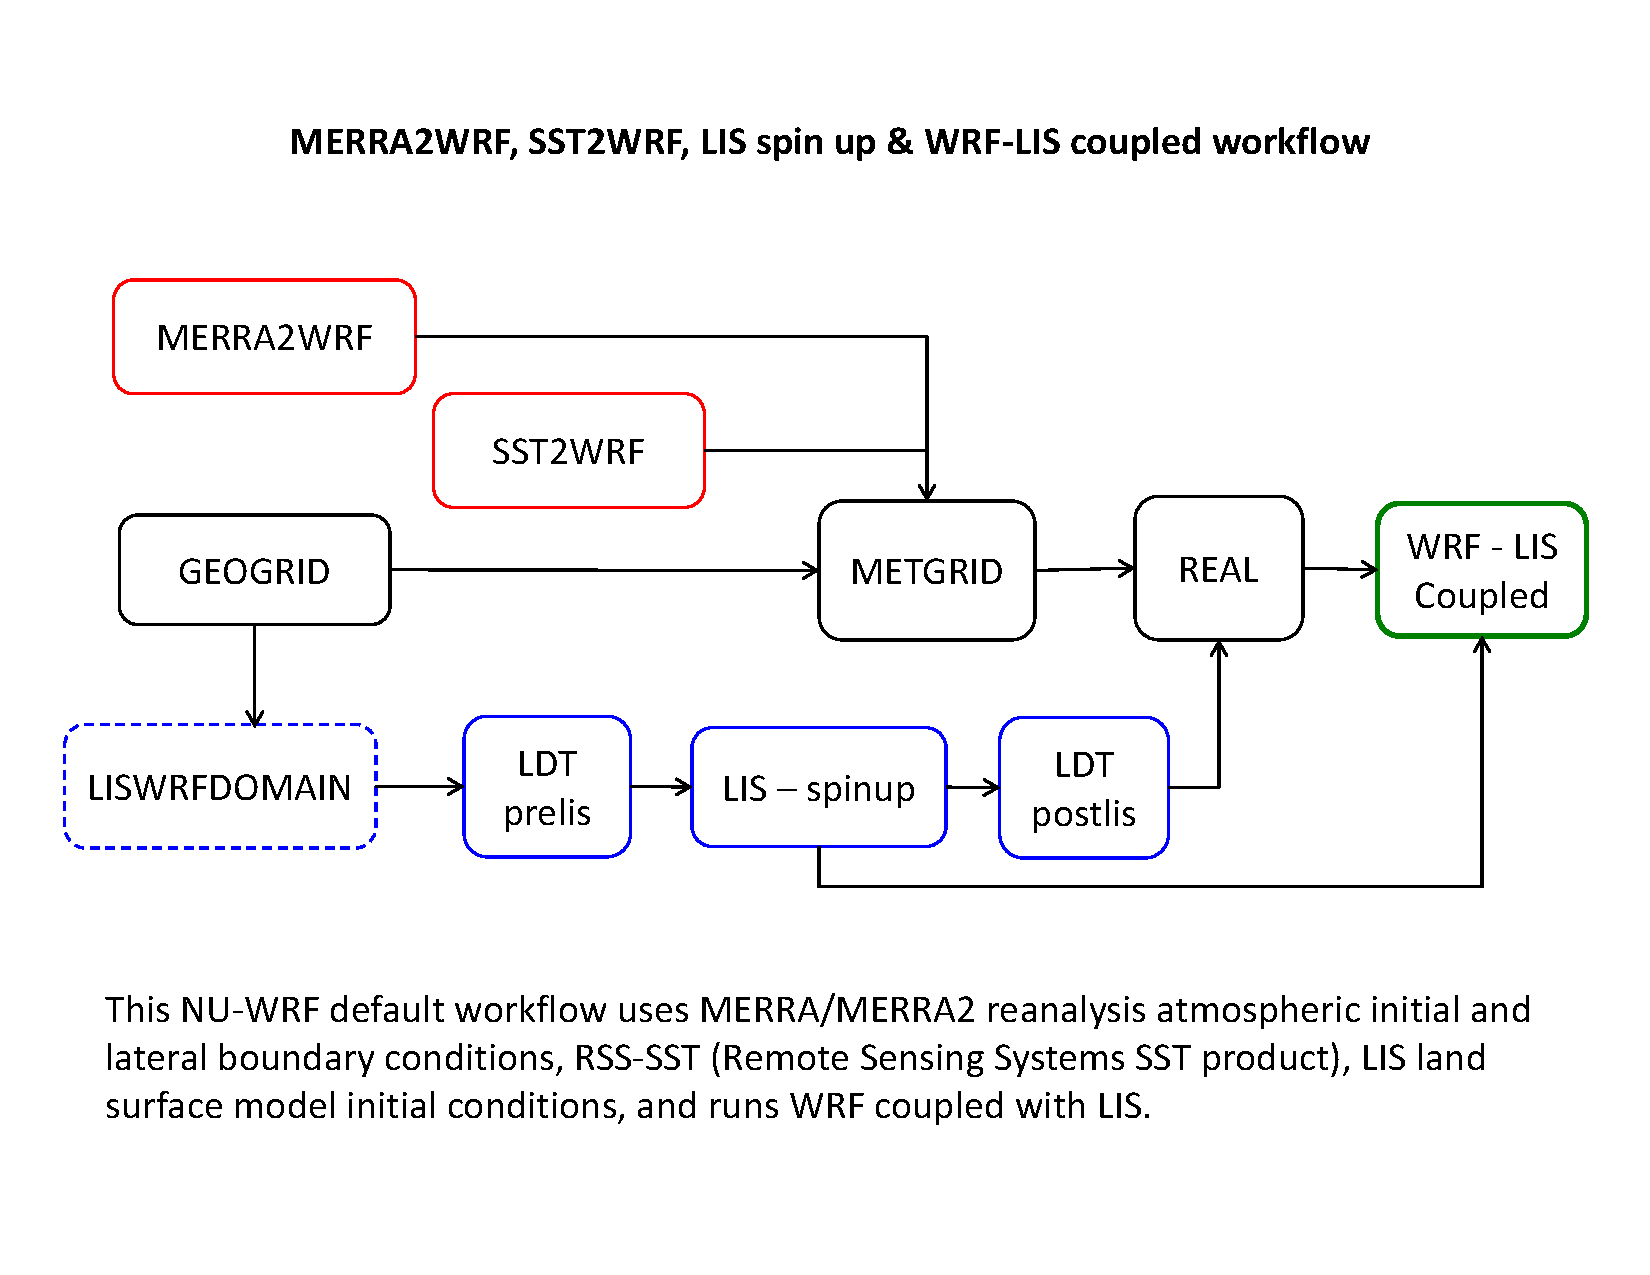
\includegraphics[scale=.4]{default-workflow.pdf}
\end{figure}

\end{frame}


%-------------------------------------------------------------------------------------------------------------------
\begin{frame}[fragile]\frametitle{Required files for default workflow}

Copy the following files to \textbf{RUNDIR}:
\begin{lstlisting}
> export RUNDIR=/discover/nobackup/<my_user_id>/scratch/default_workflow
> cp -r $PROJECTDIR/tutorial/default_workflow $RUNDIR

Where:
common.reg : shared script with settings used by other scripts.
*.reg : scripts to run pre-processors and model.
namelist* : namelist files required by executables.
\end{lstlisting}
\textbf{Note}: Unlike the "basic" workflow, we have no ungrib data. The reason is  that this workflow uses MERRA2 reanalysis data as the source of the meteorological fields.
\end{frame}

%-------------------------------------------------------------------------------------------------------------------
\begin{frame}[fragile]
\frametitle{Required script changes}
\verbatimfont{\scriptsize}%
\begin{verbatim}
> cd $RUNDIR
\end{verbatim}
Use your favorite editor to edit \textbf{common.reg} and change the values of NUWRFDIR and RUNDIR using the values set earlier.
\verbatimfont{\scriptsize}%
\begin{verbatim}
# *** Please make sure these settings are correct ***
# NUWRFDIR specifies the location of the NU-WRF source code
NUWRFDIR=<CHANGE THIS>
# RUNDIR specifies the location of the temporary run directory
RUNDIR=<CHANGE THIS>
\end{verbatim}
You may need to edit all the *.reg files' account information and other settings. However, if you belong to group s0492 then the scripts should work without any modifications.
\verbatimfont{\scriptsize}%
\begin{verbatim}
Change account to appropriate SBU charge code:
#SBATCH --account s0942 
Change if you want to change number of nodes, hasw - to run on haswell nodes:
#SBATCH --ntasks=16 --constraint=hasw
Uncomment and set according to your needs and privileges:
##SBATCH --qos=high 
Uncomment (if desired) and substitute your e-mail here:
##SBATCH --mail-user=user@nasa.gov 
\end{verbatim}

\end{frame}

%-------------------------------------------------------------------------------------------------------------------
\begin{frame}[fragile]\frametitle{A note about namelists settings}

Things to keep in mind before we run NU-WRF components.
\mbox{}\\
\begin{itemize}
\item The length of the simulations is specified in the namelist files:
\begin{itemize}
\item In namelist.wps the length is determined by start\_date and end\_date
\item In namelist.input look for start\_ and end\_ fields. 
\item The dates in both namelists must be consistent.
\end{itemize}
\item The workflow is designed to work as-is. However, if you want to run for different dates:
\begin{itemize}
\item You must get the corresponding atmospheric data for initial conditions. 
\item Yo may need to modify the namelists. For example in namelist.input, make sure end\_day - start\_day = run\_days.
\end{itemize}
\item For \textbf{any} other changes please refer to the user's guide.
\end{itemize}

\end{frame}


%-------------------------------------------------------------------------------------------------------------------
\begin{frame}[fragile]\frametitle{GEOGRID}

\scriptsize{
GEOGRID interpolates static and climatological terrestrial data (land use, albedo, vegetation greenness, etc) to each WRF grid.
\begin{itemize}
\item Input: namelist.wps
\item Output: For \emph{N} domains (max\_dom in namelist.wps), \emph{N} geo\_em files will be created.
\end{itemize}\scriptsize}    
\hrulefill\par
\scriptsize{Before running GEOGRID ensure your domain is in the right location. To do so run plotgrids\_new.ncl}
\verbatimfont{\scriptsize}%
\begin{verbatim}
> module load other/ncl-6.3.0
> ncl $NUWRFDIR/WPS/util/plotgrids_new.ncl
\end{verbatim}
\scriptsize{This is where you would edit namelist.wps to modify the domain information.
Now run GEOGRID:}
\verbatimfont{\scriptsize}%
\begin{verbatim}
> cd $RUNDIR
> sbatch geogrid.reg
\end{verbatim}
When done, check for  "Successful completion"  string in the file geogrid.slurm.out.
geogrid.log.nnnn (nnnn is the cpu number) files will also be created for tracking run failures or debugging.

\end{frame}

%-------------------------------------------------------------------------------------------------------------------
\begin{frame}[fragile]\frametitle{Use of GEOS-5 Meteorological Data}

\footnotesize{
Another  source of NU-WRF initial and lateral boundary conditions is NASA's GEOS-5 global
model. A number of dataset options exist from GEOS-5, including 
archived MERRA  and MERRA-2 reanalyses. However, there are some issues to keep in mind.\\
\mbox{}\\
First of all the GEOS-5 land surface data cannot be used to initialize WRF, due to fundamental 
differences between the GEOS-5 Catchment LSM and those in WRF. 
Thus, the GEOS-5 data in the current workflow also includes WRF-LIS. 
Second, GEOS-5 writes output in netCDF (and historically HDF4 and HDFEOS2) instead
of GRIB. And furthermore, GEOS-5 often does not output all the variables expected by
WPS.\\
\mbox{}\\
To address these issues, special preprocessing software has been developed: 
MERRA2WRF. MERRA2WRF is a program customized to process the 6-hourly
reanalyses from MERRA and MERRA-2. For 3-hourly MERRA-2 processing users must fall back 
to GEOS2WRF, which is not discussed here.}

\end{frame}

%-------------------------------------------------------------------------------------------------------------------
\begin{frame}[fragile]\frametitle{MERRA2WRF}

\footnotesize{Process MERRA2 reanalysis for WRF initial and lateral boundary conditions}.\\
\hrulefill\par
\footnotesize{
The \textbf{merra2wrf.reg} script does two things: retrieves the MERRA-2 data from the NASA GES DISC web servers; processes the downloaded data into data readable by METGRID. Note this tutorial only deals with MERRA-2 data. For MERRA data retrieval/processing please see the NU-WRF user's guide.}\\
\hrulefill\par
\begin{lstlisting}
> cd $RUNDIR
> ./merra2wrf.reg  # Not a batch script. It may take a minute or two to complete...
> cp $RUNDIR/data/merra2wrf/MERRA* $RUNDIR
\end{lstlisting}

\end{frame}

%-------------------------------------------------------------------------------------------------------------------
\begin{frame}[fragile]
\frametitle{SST2WRF}

\footnotesize{
SST2WRF processes several sea surface temperature (SST) products produced by Remote Sensing Systems (RSS; see http://www.remss.com).\\
}    
\hrulefill\par
\footnotesize{To run:}
\begin{lstlisting}
> cd $RUNDIR
> ./sst2wrf.reg  # Not a batch script. It may take a few seconds to complete...

Note that the script downloads data with  start date = 20070119 and end date = 20070120.

When done, SSTRSS* files will be created in the $RUNDIR/sstdata/mw_ir/ directory. These files must be copied to $RUNDIR before running the METGRID component. 

> cp $RUNDIR/sstdata/mw_ir/SSTRSS* $RUNDIR
\end{lstlisting}

\end{frame}

%-------------------------------------------------------------------------------------------------------------------
\begin{frame}[fragile]\frametitle{METGRID}

\footnotesize{
METGRID horizontally interpolates MERRA and SSTRSS data to the WRF domains, and combine them with the
output from GEOGRID.
\begin{itemize}
\item Input: namelist.wps, MERRA*, SSTRSS* and geo\_em* files.
\item Output: Several met\_em* files corresponding to number of intervals (interval\_seconds) in simulation length (start/end dates).
\end{itemize}
}    
\hrulefill\par
\footnotesize{To run:}
\begin{lstlisting}
> cd $RUNDIR
> sbatch metgrid.reg
\end{lstlisting}
When done, check for  "Successful completion" string in the file metgrid.slurm.out. metgrid.log.nnnn (nnnn is the cpu number) files also be created for tracking run failures or debugging.


\end{frame}

%-------------------------------------------------------------------------------------------------------------------
\begin{frame}[fragile]\frametitle{LISWRFDOMAIN (optional step)}

\footnotesize{
LISWRFDOMAIN is used to customize (and check) LDT and LIS config files so their domain(s) (grid size, resolution, and map projection) match that of WRF. It uses the output from GEOGRID  to determine the reference latitude and longitude. For this tutorial we are using pre-defined lis.config.* and ldt.config.* files that do not need to be modified (or checked). However, if you do change your GEOGRID domain  then you may need to run LISWRFDOMAIN.
\begin{itemize}
\item Input: lis.config, ldt.config and geo\_em* files.
\item Output: lis.config.new, ldt.config.new (will be identical to original config files if no changes are necessary).
\end{itemize}
}    
\hrulefill\par
\footnotesize{Example:}
\begin{lstlisting}
> cd $RUNDIR
> cp $NUWRFDIR/utils/lisWrfDomain/scripts/lisWrfDomain.py .
> ln -s $NUWRFDIR/utils/bin/lisWrfDomain.x ./EXE
> lisWrfDomain.py EXE lis.config.coldstart ldt.config.prelis ./
> lisWrfDomain.py EXE lis.config.wrf ldt.config.postlis ./
\end{lstlisting}
\scriptsize{
If the ".new" files are different then replace the original files with the "new" ones before running LDT (e.g "cp ldt.config.prelis.new ldt.config.prelis").}

\end{frame}

%-------------------------------------------------------------------------------------------------------------------
\begin{frame}[fragile]\frametitle{LDT (pre-LIS)}

\footnotesize{
LDT processes data inputs for different surface models. In this use-case we are using the Noah v3.6 land surface model.
\begin{itemize}
\item Input: ldt.config (ldt.config.prelis gets copied into ldt.config by ldt\_prelis.reg )
\item Output: lis\_input* files for each NU-WRF domain.
\end{itemize}
}    
\hrulefill\par
\footnotesize{To run:}
\begin{lstlisting}
> cd $RUNDIR
> sbatch ldt_prelis.reg

When done, check for "Finished LDT run" string in the file ldt_log_prelis.0000
\end{lstlisting}

\end{frame}

%-------------------------------------------------------------------------------------------------------------------
\begin{frame}[fragile]\frametitle{LIS}

\scriptsize{
LIS  can be run in various modes. Here we run in "retrospective" mode (a very short LIS spin up) to produce  restart and history files. The history files are used by LDT postlis and the restart files are used by WRF. 
\begin{itemize}
\item Input:  lis\_input* files for each NU-WRF domain (this is the output from LDT pre-LIS), lis.config.coldstart,  forcing\_variables\_merra2.txt, NOAH36\_OUTPUT\_LIST\_SPINUP.TBL 
\item Output: surface model output in OUTPUT/SURFACEMODEL/2007/20070120 directory. 
\end{itemize}
}    
\hrulefill\par
\scriptsize{To run:}
\begin{lstlisting}
> cd $RUNDIR
> sbatch lis.reg

When done, lis.reg copies the LIS restart/history files in OUTPUT to $RUNDIR
Check this file for successful run completion: lis.slurm.out 
lislog.nnnn files will also be created for tracking run failures or debugging.
\end{lstlisting}
\scriptsize{
For more information about LIS see \url{https://modelingguru.nasa.gov/community/atmospheric/lis}.
}
\end{frame}

%-------------------------------------------------------------------------------------------------------------------
\begin{frame}[fragile]\frametitle{LDT (post-LIS)}

\footnotesize{
After running LIS, it is necessary to rerun LDT in "NUWRF preprocessing for real" mode. This requires modifications to ldt.config to specify the static output file from LDT and the dynamic output file from LIS. Fields from both will be combined and written to a new netCDF output file for use by REAL
\begin{itemize}
\item Input: ldt.config (ldt.config.postlis gets copied into ldt.config by ldt\_postlis.reg ), LIS history files in OUTPUT directory.
\item Output: lis4real\_input* files for each NU-WRF domain.
\end{itemize}
}    
\hrulefill\par
\footnotesize{To run:}
\begin{lstlisting}
> cd $RUNDIR
> sbatch ldt_prelis.reg

When done, check for "Finished LDT run" string in the file ldt_log_postlis.0000
\end{lstlisting}

\end{frame}


%-------------------------------------------------------------------------------------------------------------------
\begin{frame}[fragile]\frametitle{REAL}

\footnotesize{
\hrulefill\par       
REAL vertically interpolates the METGRID output to the WRF grid, and creates initial and lateral boundary condition files.
\begin{itemize}
\item Input: namelist.input.real, met\_em*  files, geo\_em*, lis4real\_input* files.
\item Output: wrfinput* files (one for each domain), wrfbdy\_d01.
\end{itemize}
}    
\hrulefill\par
\footnotesize{To run:}
\begin{lstlisting}
> cd $RUNDIR
> sbatch real.reg
\end{lstlisting}
Check real.slurm.out for run completion.
If necessary check the real\_logs directory for real.rsl.out.nnnn and real.rsl.error.nnnn files.


\end{frame}

%-------------------------------------------------------------------------------------------------------------------
\begin{frame}[fragile]\frametitle{WRF}

\footnotesize{
\hrulefill\par       
Running WRF in this case is similar to the basic case, except that WRF will also read some LIS files (config, model output table) and the restarts that were produced during the "retrospective" run.\\
\begin{itemize}
\item Input: namelist.input.wrf, lis.config.wrf, NOAH36\_OUTPUT\_LIST.TBL wrfinput* files (one for each domain), wrfbdy\_d01.
\item Output: wrfout* files (one for each domain).
\end{itemize}
}    
\hrulefill\par
\footnotesize{To run:}
\begin{lstlisting}
> cd $RUNDIR
> sbatch wrf.reg
\end{lstlisting}
Check wrf.slurm.out for run completion.
If necessary check the wrf\_logs directory for wrf.rsl.out.nnnn and wrf.rsl.error.nnnn files.


\end{frame}

%-------------------------------------------------------------------------------------------------------------------
\begin{frame}[fragile]
\frametitle{Post-processing on Discover}

Using NCVIEW:

\begin{lstlisting}
WRF output files (NETCDF4) can be viewed using a special version of ncview installed on Discover:

/usr/local/other/SLES11.1/ncview/2.1.2/intel-12.1.0.233/bin/ncview <filename>
\end{lstlisting}

\end{frame}

%-------------------------------------------------------------------------------------------------------------------
\begin{frame}[fragile]
\frametitle{Post-processing on Discover}

Using RIP (NCAR graphics). Submit the \textbf{rip} job:
\begin{lstlisting}
> cd $RUNDIR
> ./rip.bash # (or use sbatch)
> idt filename.cgm # Substitute actual filename

rip.bash will run ripdp_wrfarw and rip to generate NCAR Graphics cgm files.
idt is a NCAR Graphics executable in $NCARG_ROOT/bin
Sample RIP plot specification tables are in $NUWRFDIR/scripts/rip and are looped through by rip.bash

See http://www2.mmm.ucar.edu/wrf/users/docs/ripug.htm for info on customizing plots with RIP. 
Minor changes to rip.bash may be necessary.
\end{lstlisting}

\end{frame}


